\chapter{Algorithms and software design}

This chapter describes aspects of the algorithmic concepts in SBMLsqueezer \citep{Draeger2011a}.
The focus is not on source code or concrete implementation.
The purpose of this chapter is rather to explain
\begin{enumerate*}[label=\itshape\alph*\upshape)]
  \item how the program's architecture is designed;
  \item how it makes its choices in order to select applicable rate equations for reactions of interest;
  \item which criteria the program uses in order to compare reactions in the local model to the content of \SABIO 
\citep{Wittig2012} and subsequently extracts further information.
\end{enumerate*}
For a correct use of the program an understanding of these methods is recommendable.

\section{Software architecture}

SBMLsqueezer has been planned and implemented as a modular program that follows established software design patterns, such as the Model-View-Controller pattern, and hence strictly discriminates between its (graphical or command-line) user interface, its data model, algorithms, etc.
A schematic of the program's design can be seen in \vref{fig:architecture}.
\begin{figure}[htb]
  \centering
  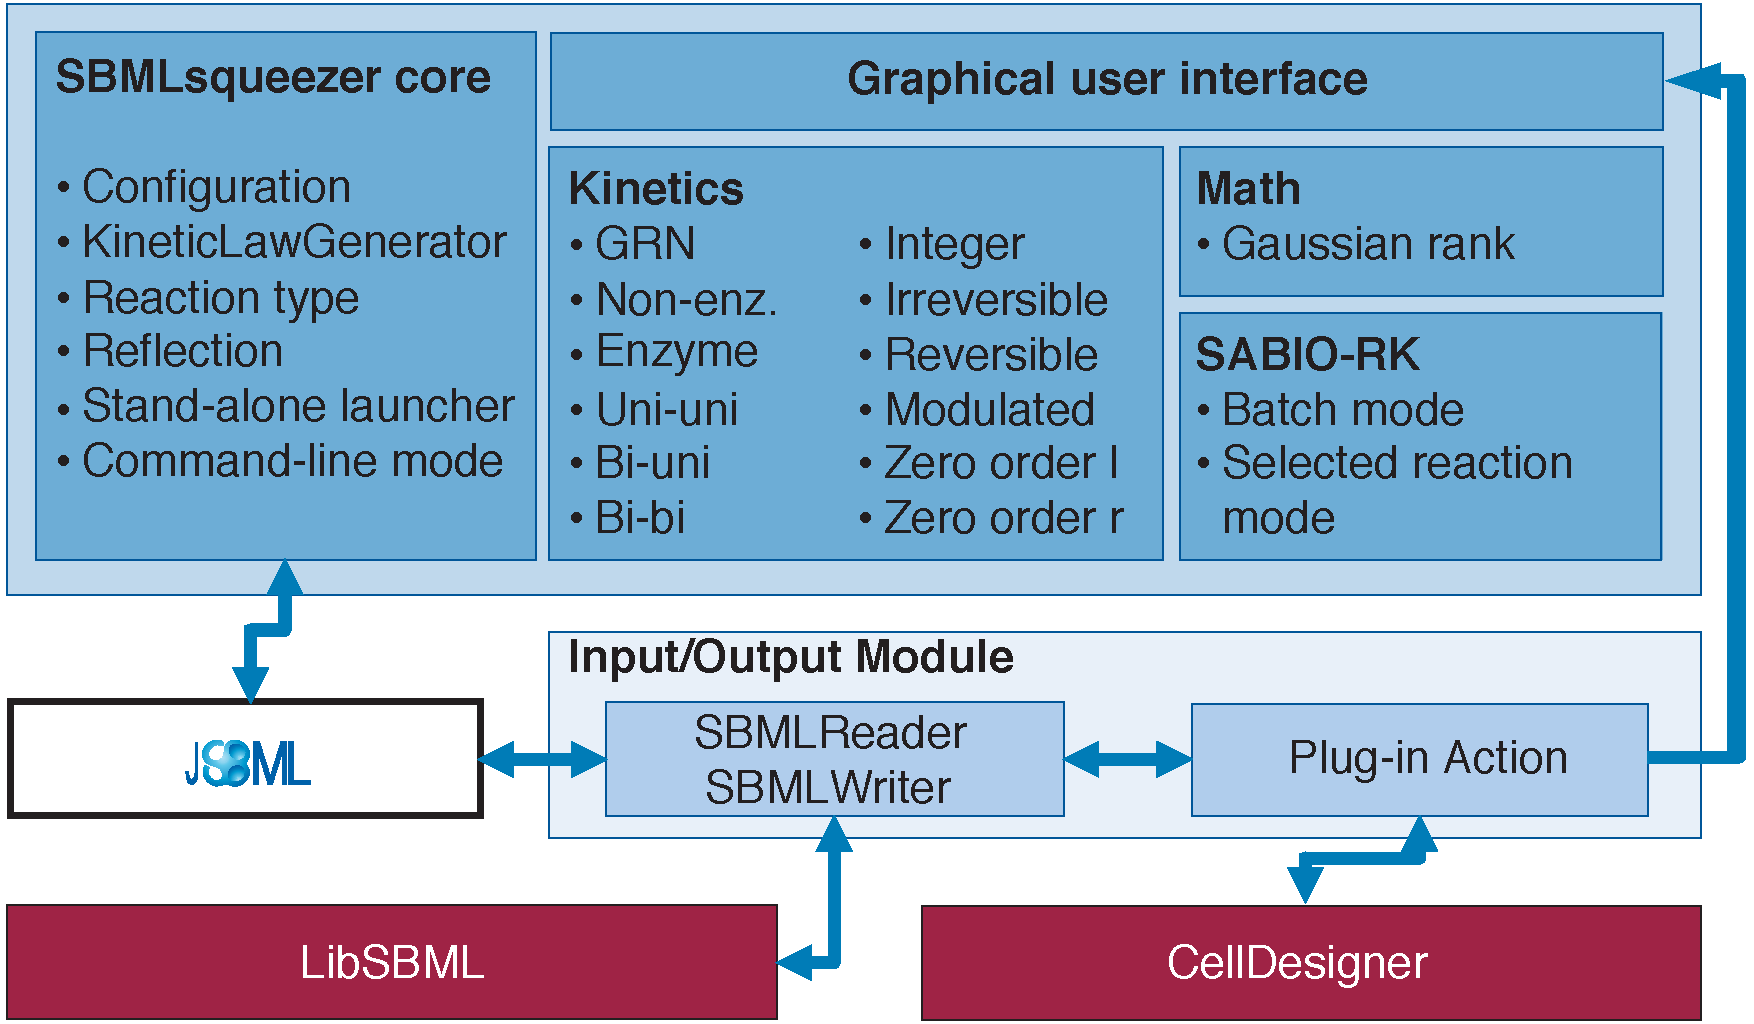
\includegraphics[width=.95\textwidth]{architecture}
  \caption[Architecture of SBMLsqueezer]{Architecture of SBMLsqueezer. The program is organized in several modules that use \JSBML as internal data structure. A compatibility layer enables the program to be used based on \libSBML, \CellDesigner, or as a stand-alone tool (also embedded in \Garuda, an online program, etc.). Modified and updated from \citet{Draeger2011a}.}
  \label{fig:architecture}
\end{figure}

SBMLsqueezer consists of a core package that provides a general infrastructure for the program.
The core deals with user preferences and command-line arguments (see \vref{chap:CMD}), and searches for online updates.
Furthermore, the core is responsible to launch the program.
This can be done in diverse ways, e.g., in command line mode, as a plug-in of \CellDesigner, as a gadget in \Garuda, etc.

The internal data structure of the program is provided by \JSBML \citep{Draeger2011b}.
Converters can read and write input \SBML documents through \libSBML \citep{Bornstein2008} or \CellDesigner's \API \citep{Funahashi2008}, or \JSBML can directly parse these files.
In this way, \JSBML acts as an abstraction layer between diverse forms of input and synchronizes all changes made by the program back to the original source.
In case that \JSBML is being directly used, the synchronization step can be omitted.

A graphical user interface can be launched from the core and has then control over all functions of the program.
For details about which functions are available and how to use the user interface, see \vref{chap:GUI}.

All implemented rate laws are gathered in the kinetics package and are grouped by twelve interfaces that are described in \vref{sec:RateLawSelection}.
For version~2, a new \SABIO package has been implemented that obtains kinetic equations from the rate law database \SABIO \citep{Wittig2012}.
A mathematics package contains an implementation of the Gaussian rank calculation, which is required for convenience rate laws \citep{Liebermeister2006}.

\section{Rate law selection}
\label{sec:RateLawSelection}

\MIRIAM \citep{Le2005, Laible2007, Juty2012, Juty2013} and \SBO annotations \citep{Courtot2011} constitute the main sources of information for SBMLsqueezer in order to make its choices.
Models can also be evaluated if no such information is given.
However, in these cases the program will most likely make different assignments compared to a fully annotated model.
When used as \CellDesigner plug-in, \SBO terms are inferred from the \CellDesigner-specific annotations of modifiers and further elements.

At first, the algorithm creates a submodel that only comprises those reactions for which rate laws are to be created.
All relevant model components, such as species, compartments, units, etc. are copied into this submodel.
Operating on this trimmed copy of the full model has the advantage that changes of the algorithm do not affect the original data structure and can be easily disregarded.
When creating this submodel, the algorithm also checks if fall-back units are defined for all components.
This is crucial in order to avoid problems in later steps.
Depending on which units are missing, it generates units for area, reaction extend, length, substance, time, and volume just as the default units in \SBML Level~2 Version~4 \citep{Hucka2008} would be defined.
All subsequent steps can hence assume that every model component has a defined unit.

The algorithm then iterates trough all reactions within the submodel and performs several pre-processing steps, before an appropriate type of rate law can be selected:
\begin{enumerate}

  \item If the user defines a list of \KEGG \citep{Kanehisa2000a} \acp{ID} for species whose contribution to rate laws should be neglected, species with such terms in their \MIRIAM annotation \citep{Le2005} are removed.
  \Cref{tab:MIRIAMignoreList} shows the predefined list of those entities.
  \item Based on their \SBO term \citep{Courtot2011} attribute all modifiers of the reaction are grouped into the following sets:
  \begin{enumerate*}[label=\itshape\alph*\upshape)]
    \item enzymes;
    \item activators;
    \item inhibitors; and
    \item non-enzyme catalysts.
  \end{enumerate*}
%If the user has decided not to implicitly consider all reactions enzyme-catalyzed, a reaction is considered a \emph{non-enzyme reaction} if either the list of enzymes is empty or there is at least one non-enzyme catalyst, or the reaction is reversible and the set of products is empty.
  Since it is not always clear if a catalyst of a reaction is an enzymatic catalyst, the user can define, which kinds of species may be considered enzymes in the specific context.
  \Cref{tab:EnzymesAndSBO} presents a list of all kinds of species that the algorithm can potentially accept as enzymes of a reaction.
The algorithm checks if any modifier of the reaction corresponds to a species with one of the \SBO terms in this list.
If the modifier is annotated as \emph{catalyst} (\href{http://identifiers.org/biomodels.sbo/SBO:0000013}{\texttt{SBO:0000013}}) and its corresponding species belongs to the list of potential enzymes, the algorithm assigns the \SBO term \emph{enzymatic catalyst} (\href{http://identifiers.org/biomodels.sbo/SBO:0000460}{\texttt{SBO:0000460}}) to the modifier.
Based on the user's selection the algorithm hence solves contradictions between the \SBO term of a modifier and the corresponding species.
\begin{SCtable}[][tb]
\begin{tabular}{ll}
\toprule
Material entity   & \SBO term\\
\midrule
\asRNA            & \href{http://identifiers.org/biomodels.sbo/SBO:0000317}{\texttt{SBO:0000317}}\\
Complex           & \href{http://identifiers.org/biomodels.sbo/SBO:0000253}{\texttt{SBO:0000253}}\\
Generic protein   & \href{http://identifiers.org/biomodels.sbo/SBO:0000252}{\texttt{SBO:0000252}}\\
Macromolecule     & \href{http://identifiers.org/biomodels.sbo/SBO:0000245}{\texttt{SBO:0000245}}\\
Receptor          & \href{http://identifiers.org/biomodels.sbo/SBO:0000244}{\texttt{SBO:0000244}}\\
\RNA              & \href{http://identifiers.org/biomodels.sbo/SBO:0000250}{\texttt{SBO:0000250}}\\
Simple molecule   & \href{http://identifiers.org/biomodels.sbo/SBO:0000247}{\texttt{SBO:0000247}}\\
Truncated protein & \href{http://identifiers.org/biomodels.sbo/SBO:0000248}{\texttt{SBO:0000248}}\\
Unknown molecule  & \href{http://identifiers.org/biomodels.sbo/SBO:0000285}{\texttt{SBO:0000285}}\\
\bottomrule
\end{tabular}
\caption[Kinds of species that can potentially act as enzymes and their top-level \SBO terms]{Kinds of species that can potentially act as enzymes and their top-level \SBO terms.
These \SBO terms correspond to the annotation of the actual species and therefore define the material classes of potential enzymes.
The terms given in this table represent the top-level terms, i.e., the algorithm also accepts each more specialized term for a specific category.
Note that the user can exclude elements from this list and therefore influence the algorithm's choices.}
\protect\label{tab:EnzymesAndSBO}
\end{SCtable}

  \item The stoichiometry of each reaction participant is analyzed in order to obtain the accumulated stoichiometry of reactants and products and to answer the question if all values are integers.
In this step the algorithm also analyzes the \SBO term \citep{Courtot2011} attribute of each reaction participant.
Further top-level \SBO terms with relevance to the algorithm can be found in \Cref{tab:FurtherRelevantSBOTerms}.
The aim of this step is to get hints if the reaction represents a transcription or translation:
  \begin{itemize}
    \item If a reactant represents a \gene or {\gene}-coding region, the reaction could be a \transcription.
    \item If the reaction involves a reactant that stands for an \RNA or \mRNA molecule it could be a \translation.
    \item If at least one modifier represents a \gene or \RNA molecule, the reaction could represent a \translation.
  \end{itemize}
  \Cref{fig:TranscriptionAndTranslation} depicts these processes in a simple schematic based on the \SBGN recommendations.
  The algorithm recognizes these these reaction patterns only based on the stoichiometry and \SBO term annotation of all participants.
%  \begin{SCfigure}
%    \includegraphics[width=.45\textwidth]{SBGN/GeneRegulatory}
%    \caption[Transcription and translation]{Transcription and translation.
%The first reaction \texttt{re1} assembles an \mRNA molecule from a source of bases.
%The presence of a specific gene enables this process.
%The resulting \mRNA molecule in turn enables the assembly of a protein from a source of amino acids.
%In a feedback inhibition loop, the protein interferes with the transcription of its corresponding gene.}
%    \label{fig:TranscriptionAndTranslation}
%  \end{SCfigure}

  \item In order to ensure that the algorithm can process each reaction within the submodel, it checks the following semantic rules:
  \begin{itemize}
    \item If a reaction involves a \gene or {\gene}-coding region as reactant or its set of reactants is \emph{empty} and all products are \RNA molecules, the reaction is recognized as \transcription.
    \item If the substrate species of a reaction are \RNA molecules or the reaction does not have any reactants and all products are forms of \protein or poly-peptide chains, the reaction is recognized as \translation.
    \item If the stoichiometry of reactants and products is unity, the reaction can only be categorized as \transcription if the only reactant is a \gene or {\gene}-coding region and it is only a valid \translation if the only reactant is an \RNA molecule.
Depending on user preferences, the algorithm can set the boundary condition for each \gene as part of this step.
  \end{itemize}
Note that a list of reactants or products is said to be \emph{empty} if either 
\begin{enumerate*}[label=\itshape\alph*\upshape)]
  \item no such list exists;
  \item no element has been assigned to this list;
  \item the stoichiometry of each element within the list is zero; or
  \item if each element in the list is annotated with an \SBO term derived from the term for \emph{empty set} (\href{http://identifiers.org/biomodels.sbo/SBO:0000291}{\texttt{SBO:0000291}}).
\end{enumerate*}
\end{enumerate}

After having reaction preprocessing and semantic checking completed, the algorithm assigns a list of applicable categories to each reaction within the submodel.
The algorithm distinguishes between the following twelve such categories, which are not necessarily exclusive:\\
\noindent
\begin{minipage}[t]{.5\textwidth}
\raggedleft
\begin{enumerate}
  \item Non-enzyme reactions (\cref{fig:NonEnzymeReactions})
  \item Gene-regulatory processes (\cref{fig:TranscriptionAndTranslation})\index{Gene}
  \item Uni-uni enzyme reactions (\cref{fig:UniUniEnzyme})
  \item Bi-uni enzyme reactions (\cref{fig:BiUniEnzyme})
  \item Bi-bi enzyme reactions (\cref{fig:BiBiEnzyme})
  \item Arbitrary enzyme reactions (\cref{fig:ArbitraryEnzyme})
\end{enumerate}
\end{minipage}% <---------------- Note the use of "%"
\begin{minipage}[t]{.5\textwidth}
\raggedleft
\begin{enumerate}
  \setcounter{enumi}{6}
  \item Integer stoichiometry reactions (\cref{fig:IntegerStoichiometry})
  \item Irreversible reactions (\cref{fig:IrreversibleReaction})
  \item Modulated reactions (\cref{fig:ModulatedReaction})
  \item Reversible reactions (\cref{fig:ReversibleReaction})
  \item Zeroth reactant order reactions (\cref{fig:ZerothReactantOrder})
  \item Zeroth product order reactions (\cref{fig:ZerothProductOrder})
\end{enumerate}
\end{minipage}\\[1em]
%\noindent
%\begin{minipage}[t]{.5\textwidth}
%\raggedleft
%\begin{enumerate}
%  \item gene-regulatory and transcriptional reactions,
%  \item zeroth reactant order reactions,
%  \item zeroth product order reactions,
%  \item reversible reactions with an optional non-enzyme catalyst,
%  \item irreversible reactions with an optional non-enzyme catalyst,
%  \item reversible enzyme-catalyzed reactions with an arbitrary number of reactants or products,
%  \item irreversible enzyme-catalyzed reactions with an arbitrary number of reactants or products,
%\end{enumerate}
%\end{minipage}% <---------------- Note the use of "%"
%\begin{minipage}[t]{.5\textwidth}
%\raggedleft
%\begin{enumerate}
%  \setcounter{enumi}{7}
%  \item reversible uni-uni type enzyme-catalyzed reactions,
%  \item irreversible uni-uni type enzyme-catalyzed reactions,
%  \item reversible bi-uni type enzyme-catalyzed reactions,
%  \item irreversible bi-uni type enzyme-catalyzed reactions,
%  \item reversible bi-bi type enzyme-catalyzed reactions, and
%  \item irreversible bi-bi type enzyme-catalyzed reactions.
%\end{enumerate}
%\end{minipage}\\[1em]
%\begin{enumerate}
%  \item gene-regulatory reactions,
%  \item zeroth reactant/product order reactions,
%  \item reversible/irreversible reactions with an optional non-enzyme catalyst,
%  \item reversible/irreversible enzyme-catalyzed reactions with an arbitrary number of reactants or products,
%  \item reversible/irreversible uni-uni type enzyme-catalyzed reactions,
%  \item reversible/irreversible bi-uni type enzyme-catalyzed reactions, and
%  \item reversible/irreversible bi-bi type enzyme-catalyzed reactions.
%\end{enumerate}
\begin{figure}[htbp]
  \centerline{
    \subfloat[A non-enzyme reaction. The ion ``I1'' catalyzes this association reaction, which can therefore not be considered enzyme catalyzed. In addition, this reaction is also modulated in a feedback inhibition loop, has an integer stoichiometry, and two reactants.]{\label{fig:NonEnzymeReactions}%
\includegraphics[width=.45\textwidth]{SBGN/IrreversibleNonEnzyme}}\hfill%
   \subfloat[Gene-regulatory processes.
Reaction \texttt{re2a} assembles an \ac{mRNA} molecule from a source of bases (transcription), enabled by the a specific gene.
This \ac{mRNA} in turn (\texttt{re2b}) enables the assembly of a protein from a source of amino acids (translation).
In a feedback inhibition loop, the protein interferes with the transcription of its own gene.]{\label{fig:TranscriptionAndTranslation}%
\includegraphics[width=.45\textwidth]{SBGN/GeneRegulatory}}}
  \centerline{\subfloat[Uni-uni enzyme reaction. This schematic conforms the classical Michaelis-Menten mechanism.]{\label{fig:UniUniEnzyme}\includegraphics[width=.45\textwidth]{SBGN/ReversibleUniUniEnzyme}}\hfill\subfloat[Bi-uni enzyme reaction. This association reaction has an integer stoichiometry.]{\label{fig:BiUniEnzyme}\includegraphics[width=.45\textwidth]{SBGN/IreversibleBiUniEnzyme}}}
  \centerline{\subfloat[Bi-bi enzyme reaction. In this example, two molecules of identical type act as reactants and also as products, respectively.]{\label{fig:BiBiEnzyme}\includegraphics[width=.45\textwidth]{SBGN/IrreversibleBiBiEnzyme}}\hfill\subfloat[Arbitrary enzyme reaction. This reversible reaction involves a feedback inhibition and a complex stoichiometry, in which an ion and two identical molecules are created from two distinct reactants.]{\label{fig:ArbitraryEnzyme}\includegraphics[width=.45\textwidth]{SBGN/ReversibleArbitraryEnzyme}}}
  \caption[Examples for general reaction categories]{Examples for general reaction categories. This figure displays example reactions in \SBGN for each of the twelve categories that are used to determine applicable rate equations.}\label{fig:ReactionCategories}%
\end{figure}
\begin{figure}[htbp]
  \ContinuedFloat
  \centerline{\subfloat[Integer stoichiometry. This reversible, enzyme-catalyzed reaction has two identical reactants and one product.]{\label{fig:IntegerStoichiometry}\includegraphics[width=.45\textwidth]{SBGN/ReversibleBiUniEnzyme}}\hfill\subfloat[Irreversible reaction. This reaction has no explicit catalyst assigned to it. Depending on user-settings, the algorithm can still consider this an enzyme-catalyzed reaction, assuming that the omission of the catalyst is for the sake of simplicity.]{\label{fig:IrreversibleReaction}\includegraphics[width=.45\textwidth]{SBGN/IrreversibleUniUni}}}
  \centerline{\subfloat[Modulated reaction. Both, a stimulator and an inhibitor interfere with this reaction.]{\label{fig:ModulatedReaction}\includegraphics[width=.45\textwidth]{SBGN/IrreversibleUniUniModulated}}\hfill\subfloat[Reversible reaction. This dissociation reaction can also be seen as an association when the equilibrium shifts to the reverse reaction.]{\label{fig:ReversibleReaction}\includegraphics[width=.45\textwidth]{SBGN/ReversibleReaction}}}
  \centerline{\subfloat[Zeroth reactant order reaction. The two product molecules lower the velocity of their own creation.]{\label{fig:ZerothReactantOrder}\includegraphics[width=.45\textwidth]{SBGN/ZerothOrderReactants}}\hfill\subfloat[Zeroth product order reaction. The reactant stimulates its own degradation.]{\label{fig:ZerothProductOrder}\includegraphics[width=.45\textwidth]{SBGN/ZerothOrderProducts}}}
  \caption[Examples for general reaction categories (continued)]{Examples for general reaction categories (continued)}\label{fig:Continued}
\end{figure}

All kinetic equations are also assigned to one or multiple of these categories.
The algorithm may now either collect all appropriate rate laws for the obtained reaction categories (types) or just the one rate law with highest priority.
While the first method allows users to interactively select rate laws of choice, the latter option is important for the automatic selection of the most appropriate equation.
\begin{SCtable}
\begin{tabular}{ll}
\toprule
Definition & \SBO term\\
\midrule
catalyst                   & \href{http://identifiers.org/biomodels.sbo/SBO:0000013}{\texttt{SBO:0000013}}\\
empty set                  & \href{http://identifiers.org/biomodels.sbo/SBO:0000291}{\texttt{SBO:0000291}}\\
enzymatic catalyst         & \href{http://identifiers.org/biomodels.sbo/SBO:0000460}{\texttt{SBO:0000460}}\\
\gene                      & \href{http://identifiers.org/biomodels.sbo/SBO:0000243}{\texttt{SBO:0000243}}\\
{\gene}-coding region      & \href{http://identifiers.org/biomodels.sbo/SBO:0000335}{\texttt{SBO:0000335}}\\
generic                    & \href{http://identifiers.org/biomodels.sbo/SBO:0000252}{\texttt{SBO:0000252}}\\
inhibition                 & \href{http://identifiers.org/biomodels.sbo/SBO:0000169}{\texttt{SBO:0000169}}\\
inhibitor                  & \href{http://identifiers.org/biomodels.sbo/SBO:0000020}{\texttt{SBO:0000020}}\\
\mRNA                      & \href{http://identifiers.org/biomodels.sbo/SBO:0000278}{\texttt{SBO:0000278}}\\
necessary stimulation      & \href{http://identifiers.org/biomodels.sbo/SBO:0000171}{\texttt{SBO:0000171}}\\
protein                    & \href{http://identifiers.org/biomodels.sbo/SBO:0000297}{\texttt{SBO:0000297}}\\
\RNA                       & \href{http://identifiers.org/biomodels.sbo/SBO:0000250}{\texttt{SBO:0000250}}\\
stimulation                & \href{http://identifiers.org/biomodels.sbo/SBO:0000170}{\texttt{SBO:0000170}}\\
stimulator                 & \href{http://identifiers.org/biomodels.sbo/SBO:0000021}{\texttt{SBO:0000021}}\\
transcriptional activation & \href{http://identifiers.org/biomodels.sbo/SBO:0000459}{\texttt{SBO:0000459}}\\
transcriptional inhibition & \href{http://identifiers.org/biomodels.sbo/SBO:0000020}{\texttt{SBO:0000020}}\\
translational activation   & \href{http://identifiers.org/biomodels.sbo/SBO:0000459}{\texttt{SBO:0000459}}\\
trigger                    & \href{http://identifiers.org/biomodels.sbo/SBO:0000461}{\texttt{SBO:0000461}}\\
translation                & \href{http://identifiers.org/biomodels.sbo/SBO:0000184}{\texttt{SBO:0000184}}\\
transcription              & \href{http://identifiers.org/biomodels.sbo/SBO:0000183}{\texttt{SBO:0000183}}\\
\bottomrule
\end{tabular}
\caption[\SBO terms with relevance for the categorization of reactions]{\SBO terms with relevance for the categorization of reactions.
The algorithm uses the \SBO terms listed in this table in order to distinguish between different types of species and modification in order to categorize a each reaction in the submodel as well as the role of individual reaction participants.
This also includes further relevant material entities of reaction participants.
Note that the algorithm always checks if the \SBO term of an element is a child of a certain reference term in order to also include all more specific sub-terms.}
\label{tab:FurtherRelevantSBOTerms}
\end{SCtable}
%
The selection of one or multiple appropriate categories and in turn suitable kinetic equations for a reaction is based on a set of defined rules, which are here summarized and simplified for the sake of better comprehensiveness.
%
The algorithm distinguishes the following three basic cases, which are not necessarily exclusive:
\begin{enumerate}
  \item The list of reactants is \emph{empty} or the reaction is reversible and the list of products is \emph{empty}.
If the reaction does neither involve {\gene}s, {\gene}-coding regions, nor \RNA molecules, then the algorithm can assign it to the  zeroth reactant order reactions if also the list of reactants is \emph{empty}, and to the zeroth product order reactions if it is reversible with an empty list of products.
If it does involve genetic components, it can be assigned to the gene-regulatory reactions depending on its directionality.

  \item The reaction has at least one reactant and if it is reversible also at least one product.
If the reaction does neither have any enzymatic catalyst nor any non-enzymatic catalyst, it is assigned to the category of non-enzyme reactions with respect to its directionality.
In case of unity stoichiometry on both sides of the reaction, and if the reaction follows the pattern of \transcription or \translation reactions, it is added to the category of {\gene}-regulatory reactions.
The pattern is satisfied if the reactant is a genetic element or an empty set and the product is an \RNA molecule or \protein.

  \item The preprocessing has revealed that the reaction belongs to enzyme kinetics.
Depending on user preferences, a reaction can also be recognized as enzyme-catalyzed process if no catalytic modifier is assigned to it.
If the reaction is reversible with at least one product, the category of arbitrary enzyme reactions is assigned.
Next, the stoichiometry and directionality of the reaction are taken into account in order to determine if the reaction also belongs to the uni-uni, bi-uni, or bi-bi reactions.
\end{enumerate}

Each reaction category is represented with one interface that can be implemented by rate laws that are applicable for this category.
Since one rate law can be useful for multiple categories, rate laws can also implement several of these interfaces.
For all categories that can be applied to a reaction, the algorithm then compiles a list of concrete kinetic equations using a concept known as \emph{reflection}.
%One post-processing step is required to modify the list of assignable rate laws.
%Not each equation can be applied to reactions that are modulated by activators or inhibitors.
%In this situation, inappropriate equations are subsequently removed from the list of equations.
%The group of those kinetic equations also implements a common interface and can therefore also be identified on run-time.
The list of applicable kinetic equations is hence generated on the fly and only based on the general reaction categories.
In this way, the program can easily be extended, because additional kinetic equations only need to declare the categories to which they can be applied and will automatically be available when the program is executed.

Additional rules apply when the algorithm compiles the list of rate laws based on reaction categories, because some rate laws can only be applied to certain combinations of categories.
For instance, the \emph{enzymatic rate law for irreversible non-modulated non-interacting uni-reactant enzymes} (\href{http://identifiers.org/biomodels.sbo/SBO:0000150}{\texttt{SBO:0000150}}) can only be applied to irreversible reactions with integer but arbitrary stoichiometry, but does not allow stimulators or inhibitors.
Thus, some categories exclude certain rate laws from being assigned to a reaction.

The user can select one default rate law for almost all categories.
No specific default rate law can be selected for the categories irreversible or reversible reactions, modulated reactions, or integer stoichiometry, because these cases mainly refine the other categories.
Instead, the selection of default rate laws is split into three major groups:
\begin{enumerate*}[label=\itshape\alph*\upshape)]
  \item {\gene}-regulatory reactions (including reactions with zeroth order reactants or products);
  \item reversible reactions; and
  \item irreversible reactions.
\end{enumerate*}
This is necessary because some rate laws can only be applied to reversible reactions, others only to irreversible reactions.

The identification of the category with highest priority works very similar.
For reactions with empty list of reactants a {\gene}-regulatory reaction has higher priority than the zeroth reactant order (but requires that the reaction follows the right pattern).
Similarly, the algorithm first tries to assign a reaction to the {\gene}-regulation category if it is reversible with an empty list of products, before assigning it to the zeroth product order reactions.
Non-enzymatic reactions have higher priority than any enzymatic reaction.
If the reaction is enzyme-catalyzed, the algorithm tries to first assign the most detailed category before it chooses an arbitrary enzyme reaction category.
Hence, the algorithm determines one category for each reaction and applies the default rate law from this category to the reaction.
In case of conflicts there are two final fall-back rate laws that can be applied if not other rate law can be selected:
\begin{enumerate*}[label=\itshape\alph*\upshape)]
  \item for non-enzyme reactions, the generalized mass-action rate law \citep{Guldberg1879, Heinrich1996}; and
  \item the convenience rate law \citep{Liebermeister2006} for any kind of enzyme-catalyzed reaction.
\end{enumerate*}
Both rate laws can be applied to reversible and irreversible reactions with arbitrary stoichiometry and can be combined with pre-factors for modification (activation or inhibition) as needed.
When creating rate laws for individual reactions, a complete list of all applicable rate laws for the reaction of interest is compiled.

When convenience rate laws are used, the algorithm prefers the simple form and applies the thermodynamically independent form only if the system does not have full column rank.
To this end, the program calculates the rank of the stoichiometric matrix using the Gaussian algorithm.
This rank check is performed only once for the given model and only executed if at least one reaction exists, for which a convenience rate law is selected.
Note that the algorithm calculates the rank for the full stoichiometric matrix and not just for the current submodel.
This is crucial, because in many cases submodels would only contain one reaction, and thus the rank would be full.

\section{Rate law creation}

Applying a rate law to the reaction means that the algorithm has to construct an abstract syntax tree, which symbolically represents the kinetic equation for the reaction.
To this end, the reaction needs to be analyzed again and all of its components need to be taken into account as relevant for the selected rate law (irreversible equations, for instance, tend to ignore effects of products).
An example for such an syntax tree can be seen in \vref{fig:AST}, which has been created for the reaction schematic displayed in \vref{fig:IrreversibleReaction}.
\begin{SCfigure}
  \includegraphics[width=.45\textwidth]{AST}
  \caption[Abstract syntax tree for an irreversible mass-action rate law]{Abstract syntax tree for an irreversible mass-action rate law. This tree represents the rate law $\nu_8 = k_8\cdot [R_1]$. The program internally constructs all equations in form of syntax trees, which can contain references to objects in the \ac{SBML} document.}
  \label{fig:AST}
\end{SCfigure}

In order to ensure unit consistency of the equation, it can be necessary to multiply or divide reactive species with/by their surrounding compartment.
User preferences and the units of the species determine if and which of those operation is required, because in \SBML, each reaction should yield units of extent per time.
Two cases need to be distinguished:
\begin{enumerate}
  \item If a species has only substance units and the user decides to bring all species to concentration units, the species must be divided by its surrounding compartment.
  \item If a species is given in concentration units and the user wants to bring all species to substance units, then a multiplication of the species with its surrounding compartment is required.
\end{enumerate}

Depending on the type of rate law that is being created and the structural composition of the reaction, a certain number of parameters needs to be constructed.
This can include forward or backward rate constants, limiting velocity rates, inhibition or stimulation constants, thermodynamic properties, and many more.
These parameters can be incorporated as local or global parameters.
To this end, the algorithm first collects all parameters in a separate list and transfers them to the submodel only when a rate law is to be applied.
Just as for species, parameter objects need to be equipped with appropriate units.
The units of many parameters also depend on the structure of the reaction, for instance, the number and units of all reactants.
Because of this connection, it can be necessary to also take the units of compartments into account when deriving the units of parameters in order to obtain extend by time units for the overall rate law.
The algorithm equips each newly created parameter with a meaningful name and identifier as well as an appropriate \SBO term.

If during this step additional units or unit definitions need to be added to the submodel, these are simplified as much as possible, annotated with a \MIRIAM identifier pointing to the Units Ontology, and equipped with meaningful names and identifiers as appropriate.
The algorithm avoids creating duplicate unit definitions by checking the model for identical existing unit definitions before adding a new one.
If possible, the newly created kinetic equation is also annotated with a corresponding \SBO term.
Due to the large number of \SBO terms that can be created by the algorithm, a comprehensive list of all cases is omitted in this document.

Whenever a kinetic equation that involves stoichiometry values is created for models in \SBML Level~3, the algorithm inserts the \ID of the corresponding species reference rather than the actual numerical value of the stoichiometry into the rate law.
This gives the advantage that model changes can be directly reflected in the rate law, hence increasing the consistency of models.
At the same time, it avoids the problem that units and meaning of single numerical values might not always be clear.

Finally, all relevant changes in the submodel are synchronized to the original model.
This includes all newly created units and unit definitions, local and global parameters, annotations, mathematical equations, reversibility flags, and boundary condition flags.
If species have been deleted from reactions, because their \MIRIAM annotation was on the ignore list, this change is skipped and not synchronized, so that the structure of the model will remain identical.
In the graphical user interface, the user can also disregard the changes.
When being used as a \CellDesigner plug-in, a special observer class synchronizes all changes from the submodel to the data model of \CellDesigner.

\section{Extraction of rate laws from \SABIO}

The extraction of rate laws from the database \SABIO requires an \SBML document and search terms as input.
All possible values for the search terms can be found in \vref{sec:SABIO_search_options}.

The algorithm first generates a \URL that is used to query the \SABIO database.
This \URL comprises the search terms and the respective \KEGG reaction \ac{ID}.
The \URL begins with the prefix \url{http://sabio.h-its.org/sabioRestWebServices/searchKineticLaws/sbml?q=}.
Each search term and its given value extend this base \URL with \texttt{keyword:value}.
If a search term is associated with a range (e.g., the temperature), the \URL is extended with \texttt{keyword:[min\textvisiblespace{}TO\textvisiblespace{}max]}.
The keywords for the terms are presented here: \url{http://sabio.h-its.org/layouts/content/docuRESTfulWeb/SearchKeyVoc.gsp}.
The operator \texttt{\textvisiblespace{}AND\textvisiblespace} connects multiple keyword-value pairs in the query.

The \URL for querying points to an \XML document for download.
In the case of success, the \XML document will be an \SBML document with all kinetic laws found for the query.
Otherwise, \SABIO returns an \XML document with an error message and the algorithm terminates with a user message.

Just like for the \emph{de novo} creation of rate laws the algorithm can either process all reactions within the \SBML document or one particular reaction.
To this end, the algorithm creates one query \URL for each reaction, for which a rate law should be extracted from \SABIO.
After obtaining an \SBML document from \SABIO, the algorithm extracts all kinetic laws from the \SBML document and tries to match all elements contained in a kinetic law to elements in the input network. 
This matching is based on the \MIRIAM annotations of model components and involves the search for one corresponding
\begin{itemize}
  \item species in the local model for each species that participates in the kinetic law.
  \item compartment in the local model for each compartment addressed in the kinetic law (this can be the compartment of a participating species or the reaction itself can have a compartment assigned to it).
  \item reaction in the local model for each reaction in the kinetic law.
  \item species reference for each species reference in the kinetic law within each such identified local reaction. 
This species reference needs to refer to a species with an annotation similar to that of the species referenced by the species reference in the found rate law.
\end{itemize}
In this context, an annotation of two \SBML elements is considered similar and hence these elements are considered a \emph{match} if both have \emph{controlled vocabulary terms} in common that are linked through qualifiers \emph{has version} or \emph{is}.

In the batch mode, the algorithm always selects the first kinetic law in the query results for which all elements can be matched to respective elements in the model.
The algorithm adds this rate law to the reaction.
This merging involves
\begin{enumerate}
  \item substituting all elements in the found kinetic law with the matched elements in the model; and
  \item adding unit definitions, function definitions, global and local parameters contained in the kinetic law to the model.
\end{enumerate}

Since this algorithm mainly operates on models obtained from \SABIO it is not necessary to create a submodel copy of the local model beforehand (as this is done for the \emph{de novo} creation of rate laws).
Changes are only applied upon user agreement or in batch mode.
This is done by merging required components from the downloaded model into the local model.
For this reason, the local model does not change, before rate laws are applied.

When rate laws are obtained from \SABIO for individual reactions, the algorithm presents a list of all rate laws found for the given query to the user, who can then select the most appropriate equation.
In cases when the selection of the first law with a successful matching does not lead to a satisfying result, the single reaction mode might yield better results.


% 03_Troubleshooting
